\chapter{Materiais e Métodos}



 Devido a área de estudos de ligas de alta entropia ser algo relativamente novo, o número de bases de dados publicamente disponíveis para uso ainda é escasso. Para o atual trabalho foi escolhida uma base de dados disponibilizada em \cite{borg2020expanded} %\cite{qiao2021focused} e \cite{couzinie2018comprehensive}%.
 Essa base representa as características de diferentes ligas de alta entropia, sua composição química, microestrutura, tratamento mecânico, entropia de mistura, raio atômico e outras variáveis que serão descritas a seguir.


\section{Variáveis Utilizadas}\label{sec:MAT_MET_SEC_A}

Na base de dados foram utilizadas as características:


\begin{itemize}
    \item $\Delta S_{mix}$ :  Entropia de mistura
    \item $a_{m}$ :  Constante de rede calculada pela regra das misturas
    \item $ T_{m}$ :  Temperatura de fusão calculada pela regra das misturas
    \item $\chi_{m} $:  Média da eletronegatividades de Pauling
    \item $r_{m} $ :  Raio atômico médio
    \item $\Delta \chi$ :  Média das eletronegatividades de Pauling
    \item $\Delta a$ :  Diferença das das constantes de rede
    \item $\Delta T$ :  Diferença das temperaturas de fusão
    \item $\Delta r$ : Diferença no raio atômico
\end{itemize}

Uma análise exploratória dos dados foi realizada para compreender a estrutura, dispersão, e a correlação entre as variáveis antes que qualquer tipo de tratamento, 

\section{Tratamento dos dados}\label{sec:MAT_MET_SEC_B}
\subsection{Tipologia das variáveis}\label{sec:MAT_MET_SEC_B_SUB_A}

Após realizar uma análise exploratória dos dados, verificou-se a presença de variáveis categóricas ou qualitativas nominais, isto é, dados que possuem uma descrição e não um valor numérico contínuo\cite{pinheiro2013probabilidade}. Para tornar esses dados algebricamente manipuláveis, foi realizado um processamento em que as variáveis categóricas são agrupadas, cada grupo recebe um valor numérico, e assim temos as qualitativas nominais como variáveis numéricas discretas\cite{pinheiro2013probabilidade}. 

\subsection{Tratando os dados vazios}\label{sec:MAT_MET_SEC_B_SUB_B}

O conjunto de dados possui valores do tipo ``vazio'' nos atributos de composição química, para um algoritmo de aprendizado de máquina não é possível ajustar uma curva com a presença desse tipo de dado. Neste caso, para tornar esses dados algebricamente manipuláveis, os valores foram substituídos por zero, por exemplo, uma liga de Co1Fe1Ni1 possui apenas informações para os elementos Co, Fe e Ni, sendo assim para essa liga, os outros parâmetros de composição química como por exemplo Al, Cu, Mn recebem o valor zero, ao invés de uma informação vazia. Atribuir por padrão o valor zero nas composições químicas é completamente aceitável, pois é o mesmo que descrever a ausência deste elemento para essa liga.

\subsection{Tratando os dados duplicados}\label{sec:MAT_MET_SEC_B_SUB_C}
Dados faltantes são de certa forma um problema, e também deve-se observar a presença de dados redundantes, isto é, dados duplicados. Quando temos uma quantidade significante de dados repetidos, estamos prejudicando a análise. Após remover os dados duplicados, foi observado um aumento significante da acurácia e uma redução do desvio padrão.

Foi feita uma avaliação inicial para verificar o impacto, positivo ou negativo da remoção dos dados duplicados, os resultados foram gerados utilizando o modelo Random Forest Classifier com as configurações padrão do modelo, também foi realizada a validação cruzada ao treinar o modelo. Os resultados obtidos estão nas Tabelas \ref{table:relatorio_todos_dados} e \ref{table:relatorio_sem_duplicados}. Onde temos a precisão, .

\begin{table}[htb]
\centering
\caption{Conjunto de dados completo, n=589 }
\begin{supertabular}{l|c|c|c|c}
\hline
{ microestruturas } & { precision } & { recall } & { f1-score } & { support }\\\hline
{ BCC } &           {0.718750} &  {0.746753} & {0.732484} &  {154.000000}\\\hline
{ BCC ++ } &        {0.478873} &  {0.395349} & {0.433121} &  {86.000000}\\\hline
{ BCC B2 } &        {0.460000} &  {0.547619} & {0.500000} &  {42.000000}\\\hline
{ FCC } &           {0.717949} &  {0.761905} & {0.739274} &  {147.000000}\\\hline
{ FCC ++ } &        {0.587302} &  {0.445783} & {0.506849} &  {83.000000}\\\hline
{ FCC BCC } &       {0.490566} &  {0.577778} & {0.530612} &  {45.000000}\\\hline
{ OTHER } &         {0.444444} &  {0.500000} & {0.470588} &  {32.000000}\\\hline
{ accuracy } &      {0.616299} &  {0.616299} & {0.616299} &  {0.616299}\\\hline
{ macro avg } &     {0.556841} &  {0.567884} & {0.558990} &  {589.000000}\\\hline
{ weighted avg } &  {0.614215} &  {0.616299} & {0.612443} &  {589.000000}\\\hline
\end{supertabular}
    \legend{}
    \label{table:relatorio_todos_dados}
\end{table}

\pagebreak


\begin{table}[htb]
\centering
\caption{Conjunto de dados sem duplicados, n=382}
\begin{supertabular}{l|c|c|c|c}
\hline
{ microestruturas } & { precision } & { recall } & { f1-score } & { support }\\\hline
{ BCC } &           {0.738739} & {0.766355} & {0.752294} & {107.000000}\\\hline
{ BCC++ } &        {0.529412} & {0.409091} & {0.461538} & {66.000000}\\\hline
{ BCC B2 } &        {0.405405} & {0.483871} & {0.441176} & {31.000000}\\\hline
{ FCC } &           {0.512500} & {0.661290} & {0.577465} & {62.000000}\\\hline
{ FCC++ } &        {0.641026} & {0.471698} & {0.543478} & {53.000000}\\\hline
{ FCC BCC } &       {0.545455} & {0.571429} & {0.558140} & {42.000000}\\\hline
{ OTHER } &         {0.550000} & {0.523810} & {0.536585} & {21.000000}\\\hline
{ accuracy } &      {0.589005} & {0.589005} & {0.589005} & {0.589005}\\\hline
{ macro avg } &     {0.560362} & {0.555363} & {0.552954} & {382.000000}\\\hline
{ weighted avg } &  {0.593618} & {0.589005} & {0.586258} & {382.000000}\\\hline
\end{supertabular}
    \legend{}
    \label{table:relatorio_sem_duplicados}
\end{table}


Após remover os dados duplicados, foi realizada uma análise de correlação dos dados, o modelo de correlação escolhido foi o de Kendalls's, uma vez que é mais robusto e melhor para pequenas amostras e com possíveis outliers.

\begin{figure}[ht]
    \centering
    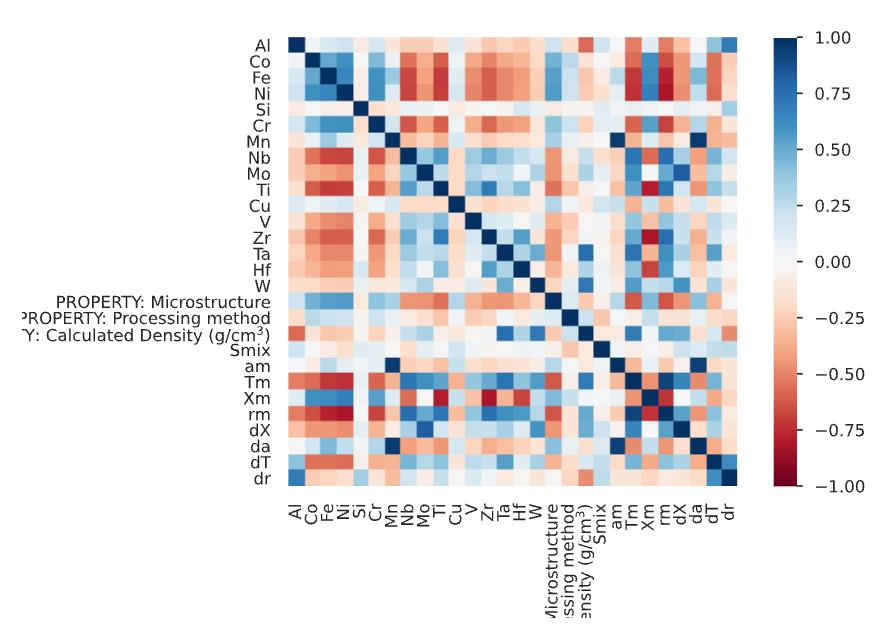
\includegraphics[height=8cm]{estrutura_dos_dados.jpg} 
    \caption{Correlação de Kendall's }
    \label{fig:kendals_correlacao_sem_duplicados}
\end{figure}
\FloatBarrier


\subsection{Normalização dos dados}\label{sec:MAT_MET_SEC_B_SUB_D}

Após remover os itens duplicados co conjunto de dados, foi verificado a redução da acurácia do modelo, que é justificado devido a algum tipo de overfitting do modelo, a ocorrência de dados duplicados são os principais responsáveis por ``viciar'' o modelo a determinado tipo de dado.

A próxima etapa será executada com o conjunto de dados sem os dados duplicados. Primeiramente precisamos subdividir as variáveis em normalizáveis e não normalizáveis. As variáveis normalizáveis são as que possuem alguma possibilidade de conter dados outliers, isto é, dados fora de um intervalo interquartil. Assim, os dados não normalizáveis foram os dados de composição química, uma vez que a composição química do conjunto de dados é definida por porcentagem, e o método de processamento, pois é uma variável categórica.

Os outros dados que são variáveis contínuas, passaram por um processo de normalização. 


\begin{table}[htb]
\centering
\caption{Conjunto de dados normalizados}
\begin{supertabular}{l|c|c|c|c}
\hline
{ microestruturas } & { precision } & { recall } & { f1-score } & { support }\\\hline
{ BCC } &           {0.692308} & {0.757009} & {0.723214} & {107.00000}\\\hline
{ BCC++ } &         {0.577778} & {0.393939} & {0.468468} & {66.00000}\\\hline
{ BCC B2 } &        {0.428571} & {0.580645} & {0.493151} & {31.00000}\\\hline
{ FCC } &           {0.513158} & {0.629032} & {0.565217} & {62.00000}\\\hline
{ FCC++ } &         {0.641026} & {0.471698} & {0.543478} & {53.00000}\\\hline
{ FCC BCC } &       {0.558140} & {0.571429} & {0.564706} & {42.00000}\\\hline
{ OTHER } &         {0.500000} & {0.476190} & {0.487805} & {21.00000}\\\hline
{ accuracy } &      {0.583770} & {0.583770} & {0.583770} & {0.58377}\\\hline
{ macro avg } &     {0.558711} & {0.554278} & {0.549434} & {382.00000}\\\hline
{ weighted avg } &  {0.589602} & {0.583770} & {0.579581} & {382.00000}\\\hline
\end{supertabular}
    \legend{}
    \label{table:relatorio_normalizados}
\end{table}


\begin{table}[htb]
\centering
\caption{Conjunto de dados com sobre amostragem}
\begin{supertabular}{l|c|c|c|c}
\hline
{ microestruturas } & { precision } & { recall } & { f1-score } & { support }\\\hline
{ BCC } &           {0.819444} & {0.797297} & {0.808219} & {74.000000}\\\hline
{ BCC++ } &         {0.783784} & {0.783784} & {0.783784} & {74.000000}\\\hline
{ BCC B2 } &        {0.835443} & {0.891892} & {0.862745} & {74.000000}\\\hline
{ FCC } &           {0.826087} & {0.770270} & {0.797203} & {74.000000}\\\hline
{ FCC++ } &         {0.794872} & {0.837838} & {0.815789} & {74.000000}\\\hline
{ FCC BCC } &       {0.847222} & {0.824324} & {0.835616} & {74.000000}\\\hline
{ OTHER } &         {0.905405} & {0.905405} & {0.905405} & {74.000000}\\\hline
{ accuracy } &      {0.830116} & {0.830116} & {0.830116} & {0.830116}\\\hline
{ macro avg } &     {0.830323} & {0.830116} & {0.829823} & {518.000000}\\\hline
{ weighted avg } &  {0.830323} & {0.830116} & {0.829823} & {518.000000}\\\hline
\end{supertabular}
    \legend{}
    \label{table:relatorio_oversampled}
\end{table}



\begin{table}[htb]
\centering
\caption{Conjunto de dados com sobre amostragem homologados}
\begin{supertabular}{l|c|c|c|c}
\hline
{ microestruturas } & { precision } & { recall } & { f1-score } & { support }\\\hline
{ BCC } &           {0.857143} & {0.909091} & {0.882353} & {33.000000}\\\hline
{ BCC++ } &         {1.000000} & {0.625000} & {0.769231} & {16.000000}\\\hline
{ BCC B2 } &        {0.700000} & {0.777778} & {0.736842} & {9.000000}\\\hline
{ FCC } &           {0.562500} & {0.500000} & {0.529412} & {18.000000}\\\hline
{ FCC++ } &         {0.818182} & {0.500000} & {0.620690} & {18.000000}\\\hline
{ FCC BCC } &       {0.541667} & {1.000000} & {0.702703} & {13.000000}\\\hline
{ OTHER } &         {0.666667} & {0.750000} & {0.705882} & {8.000000}\\\hline
{ accuracy } &      {0.730435} & {0.730435} & {0.730435} & {0.730435}\\\hline
{ macro avg } &     {0.735165} & {0.723124} & {0.706730} & {115.000000}\\\hline
{ weighted avg } &  {0.763591} & {0.730435} & {0.726443} & {115.000000}\\\hline
\end{supertabular}
    \legend{}
    \label{table:relatorio_oversampled_homolog}
\end{table}


Objetivos:
através de clusterização, o objetivo do trabalho proposto é a classificação de uma liga e a predição da tensão de escoamento e da fase presente na liga utilizando como parâmetro de entrada a composição química da liga e a sua densidade.

De início serão feitas diversas simulações com diferentes tipos de modelos cada um com sua particularidade. Com auxílio de indicadores estatísticos será decidida qual melhor ferramenta utilizar.

Primeiro passo será a análise exploratória dos dados, verificando quais tipos de dados presentes na base, ocorrência de campos ausentes ou com dados outliers.

Em seguida serão utilizados diferentes modelos disponíveis na biblioteca python scikit-learn e então compará-los com diferentes medidas estatísticas, matriz de confusão, acurácia, precisão. 

O conjunto de dados contem aproximadamente 600 amostras, com os seguintes parâmetros: nome das ligas, a composição química de cada elemento, e alguns dados empíricos como entropia de mistura, módulo de Young, microestrutura, densidade entre outros.


\section{Comparando Modelos}\label{sec:LABEL_CHP_5_SEC_A}

A biblioteca scikitlearn do python disponibiliza alguns modelos para treinar e classificar um conjunto de dados. Foram escolhidos 6 modelos para fazer essa comparação inicial. São eles GradientBoostingClassifier, RandomForestClassifier, MLPClassifier, KNeighborsClassifier, SVC e  DecisionTreeClassifier. 





Ao analisar o conjunto de dados, foi observado que os elementos químicos hora estão presentes pra algum grupos de ligas, e hora estão presentes em outros grupos. 
No primeiro treino e teste a acurácia apresentou resultados de aproximadamente 60\%, considerando um modelo geral para todo o conjunto de dados, porém o desvio padrão estava acima dos 10\%.

Após clusterizar os dados, foi gerado um modelo para cada grupo, e assim verificado a acurácia e o desvio padrão. Foram feitos agrupamentos para 3,5 e 7 clusters. 
os resultados estão na Tabela \ref{quad:clusters_acuracia}, utilizando o cross validation com 10 partiçções foram obtidos esses resultados:


\begin{table}[htb]
\centering
\caption{Clusters: 3 }
\begin{supertabular}{|c|c|c|c|c|}
\hline
{ cluster }&{ $\mu$(acurácia) }&{ $\sigma$(acurácia) }&{ qtde }&{ $(\%)$ }\\\hline
{ 1 } &
{ 0.785 } &
{ 0.123 } &
{ 135 } &
{ 28.7 }\\\hline
{ 2 } &
{ 0.704 } &
{ 0.081 }& 
{ 247 } &
{ 52.4 }\\\hline
{ 3 } &
{ 0.921 } &
{ 0.072 }&
{ 89 } &
{ 18.9 }\\\hline
\end{supertabular}
    \legend{}
    \label{quad:clusters_acuracia}
\end{table}





Variaveis experimentais importantes:
medir a resistencia mecanica - dizer a temeperatura

prever a fase - dizer como material foi sintetizado ( fundido, Tratamento térmico, fundição, sinterização .. ) 

\pagebreak


coeficiente de variacao 

https://www.cpt.com.br/artigos/em-estatistica-como-saber-se-um-desvio-padrao-e-grande-ou-pequeno

Atualmente temos para um conjunto de dados dividido em 10 partes uma acuracia media de $ 56\% $, e um desvio padrao de $ 9 \%$

O foco agora é encontrar um padrão de dados onde a acuracia e desvio padrao do modelo se comportem melhor, isto é, para alguns casos temos um pouco de overfiting no modelo, ocasionando discrepancias na previsao quando a liga possui uma gama de elementos que de certa forma é um outlier para o conjunto geral dos dados.









\section{Tratamento dos dados}\label{sec:MAT_MET_SEC_C}

Para o conjunto de dados utilizado, não será avaliado o tipo de teste (tração/compressão) nem a tensão de escoamento, sendo assim, essas colunas foram removidas do conjunto de dados.

Além disso, após remover essas colunas foi feita uma limpeza de linhas duplicadas, sendo assim de um total de 589 dados, sobraram 382. Isso permitiu que o desvio padrão do treinamento do modelo fosse reduzido, uma vez que com dados repetidos, estava ocasionando overfitting no modelo.



\clearpage
\section{Exemplos de Citações}
{\centering\bfseries\color{red}
Exemplos de Citações
\par}

{\centering\bfseries\color{red}
Citação direta:
\par}

\bigskip

Citações diretas de até 3 linhas, devem iniciar e terminar por aspas duplas.\\

Se o texto original já contiver aspas duplas, substituí-las por aspas simples. A indicação da fonte da citação pode
estar inserida no texto ou após a citação.\\

\bigskip

{\color{red}
Exemplo:}

\bigskip

Segundo Castro (2001, p. 23): {\textquotedbl}Os deveres da conduta do anestesiologista constituem predicados importantes
quando se quer avaliar a qualidade do procedimento.{\textquotedbl}\\

\bigskip

{\color{red}
ou}

\bigskip

{
{\textquotedbl}A expressão 'furiosa' dessa estátua de que fala Rebelais, corresponde também à realidade.{\textquotedbl}
(BAKHTIN, 1987, p. 89).}

\bigskip

{\centering\bfseries\color{red}
Citação Direta com mais de três linhas:
\par}

\bigskip

As citações diretas, no texto, com mais de três linhas, devem ser
destacadas com recuo de 4 cm da margem esquerda, com letra menor que a do texto utilizado e sem as aspas. A indicação da fonte da citação pode estar inserida no texto ou após a citação. \\ 

\bigskip

{\color{red}
Exemplo:}
\bigskip
Sobre mercado financeiro, Fortuna (1996, p. 15) considera:\\
\bigskip

\begin{citacao}
O mercado financeiro permite que um agente econômico qualquer, sem perspectivas de aplicação, em algum empreendimento
próprio, da poupança que é capaz de gerar, seja colocado em contato com outro, cujas perspectivas de investimento
superam as respectivas disponibilidades de poupança.\\
\end{citacao}

\bigskip
A seguir uma citação em inglês:\\

\begin{citacao}[english]
This text is an example in English language in italic with correct hyphenation. This text is an example in English language in italic with correct hyphenation. This text is an example in English language in italic with correct hyphenation.
\end{citacao}
\bigskip

\clearpage{\centering\bfseries\color{red}
Citação Indireta:
\par}

\bigskip

Não se utilizam aspas para esse tipo de citação, nem a(s) página(s) de onde foi extraída a ideia.\\

\bigskip

{\color{red}
Exemplo:}

\bigskip
esse aqui 

A bíblia começou a ser escrita no ano 1.000 a.C. e foi finalizada em 100 d.C., com a morte do último apóstolo, São João, levando aproximadamente 1.150 anos para ser concluída \cite{book:GHELLER}.\\


\bigskip

{\centering\bfseries\color{red}
Citação de Citação:
\par}

\bigskip

A indicação da fonte é feita pelo sobrenome do autor da obra citada (não consultada), ano, seguido da expressão latina apud. Após, indica-se o sobrenome do autor da obra consultada, seguido do ano de publicação, precedido por vírgula. Quando for citação direta incluir a(s) página(s) após a data de publicação, precedida de vírgula.\\

\bigskip

{\sffamily
\textrm{\textcolor{red}{Exemplo no texto}}\textrm{:}}

\bigskip

{\sffamily
\textrm{citado por }}

\bigskip

{\sffamily
\textrm{Segundo Marques e Ribeiro}\footnote{\ MARQUES, Alberto; RIBEIRO, \textbf{Angela. As fazendas agrícolas}. São
Paulo: Ática, 2000. 350 p.}\textrm{ (2000 }\textrm{\textcolor{black}{apud }}\textrm{OLIVEIRA, 2001), \apudonline {art:PRADO}{book:AMADO} o Serviço de
Atenção Médico-Sanitário da Suécia tem uma tradição de mais de cem anos. }}

\bigskip

{\color{red}
ou}

{\sffamily
\textrm{\textcolor{red}{Em nota de rodapé}}\textrm{:}}

\bigskip

{\centering\bfseries\color{red}
Indicação da Citação:
\par}

\bigskip

{\sffamily
\textrm{Se a indicação da fonte da citação estiver incluída na frase, a mesma deve aparecer apenas com a inicial
maiúscula seguida de parênteses, com a data de publicação do }\textrm{documento. Quando for citação direta incluir a(s)
página(s) após a data de publicação, precedida de vírgula.}}

\bigskip

{\color{red}
Exemplo com autor pessoal:}

\bigskip

Segundo Fonseca(2004, p. 36): {\textquotedbl}Se não houver mecanismos jurídicos que assegurem a proteção dos direitos
humanos, esse valor não será concretizado pelo Poder Público.{\textquotedbl}\\

\bigskip

{\sffamily
\textrm{\textcolor{red}{Exemplo com dois autores: }}}

\bigskip

Tonetto e Reck (2001, p. 134) destacam: {\textquotedbl}Este autoconhecimento pressupõe conhecer seus limites
[...]{\textquotedbl} \\

\bigskip

{\color{red}
Exemplo com mais de três autores:}

\bigskip

Neste contexto, Couto e outros (2004, p. 52) destacam que: {\textquotedbl}No capitalismo não é a simples ausência do
patrão que promove a superação do despotismo da divisão laboral.{\textquotedbl}\\

\bigskip

{\sffamily
\textrm{\textcolor{red}{Exemplo com autor institucional: }}}

\bigskip

De acordo com a Pontifícia Universidade Católica do Rio Grande do Sul (2001, p. 24): {\textquotedbl}[...] no horizonte 2001/2010, o esforço estratégico da PUCRS será centrado em sete áreas estratégicas [...]{\textquotedbl}\\

\bigskip

{\color{red}
Exemplo sem autor(es), com a entrada pelo título:}

\bigskip

Segundo o Guia de clareamento dental (1996, p. 8): {\textquotedbl}A causa mais comum do escurecimento dental é o tratamento endodôntico realizado de modo inadequado e sem os cuidados técnicos.{\textquotedbl}\\

\bigskip

{\color{red}
Exemplo sem autor(es), com a entrada pelo título que inicia por artigo:}

\bigskip

O movimento social, com o intuito de realizar uma transformação social, é uma das tarefas mais importantes da atualidade
(O COOPERATIVISMO..., 2002).\\

\bigskip

As citações a seguir foram colocadas para que as referências aparecessem na bibliografia. Como exemplo temos os livro de Jorge Amado \cite{book:AMADO}  \cite{book:AMADO2}, e este autor que desconheço \cite{book:OHANSSON}, além de \cite{book:ENGEL} e um artigo \cite{art:PRADO}. Notem que é gerado um link hipertexto no documento em PDF.
